\subsection{Тестирование производительности}

Производительность будет тестироваться с помощью встроенного в SolidWorks средства
SOLIDWORKS Performance Test. В этом тесте проверяется производительность системы в
типичных для SolidWorks задачах. Тестирование будет производиться на следующих
конфигурациях аппаратного обеспечения:
\begin{enumerate}
    \item Компьютеры, используемые на кафедре КПРС. Тест производится для оценки
        изначальной производительности системы.
    \item Используемый сервер. Включен в тест для оценки чистой производительности
        сервера, а также для оценки падения производительности на клиентских машинах.
    \item Разработанные тонкие клиенты. Тест проводится на 2 тонких клиентах и сервере
        одновременно для исследования влияния клиентов друг на друга. Тест отражает
        сценарий использования системы под нагрузкой.
    \item Тонкий клиент, тест запущен только на одном устройстве для верификации данных.
        Результаты должны быть идентичны пункту 2 (в пределах погрешности).
        Необходимо сравнить результаты с используемыми сейчас компьютерами для оценки
        изменения производительности всей системы.
\end{enumerate}

\begin{figure}[h]
    \center
    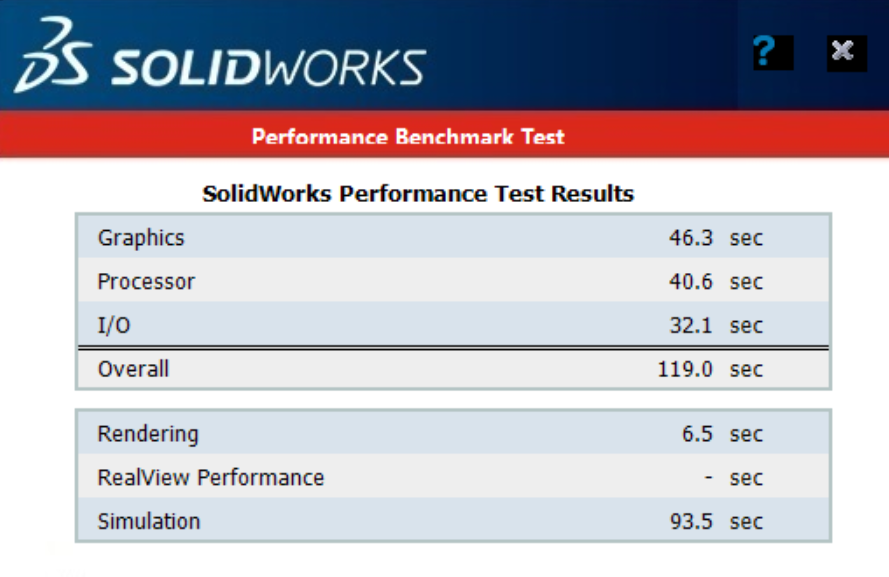
\includegraphics[height=8cm]{server_perf}
    \caption{Пример результата Solidworks Performance Test (2 конфигурация)}
    \label{pic:server_perf}
\end{figure}

Все тесты выполнялись 3 раза, результаты усреднены и представлены в сравнительной
таблице~\ref{tab:perf_comp}. Данные показывают время выполнения одного теста и
представлены в секундах, меньше — лучше.

\begin{table}[h]
    \centering
    \caption{Сравнение производительности, средние значения}
    \label{tab:perf_comp}
    \begin{tabu}to \linewidth{XX[1,c,m]X[1,c,m]X[1,c,m]X[1,c,m]}
        \toprule
        Конфигурация & 1     & 2    & 3 & 4    \\
        \midrule
        Графика      & 52,1  & 48,3 &   & 46,5 \\
        Процессор    & 51,0  & 40,4 &   & 39,4 \\
        Ввод-вывод   & 31,7  & 30,8 &   & 33,0 \\
        Рендеринг    &  7,6  &  7,2 &   & 6,8  \\
        Симуляция    & 105,0 & 92,0 &   & 95,4 \\
        \bottomrule
    \end{tabu}
\end{table}


